%\documentclass[A4,12pt]{article}
\documentclass[letterpaper,12pt]{article}
\usepackage{epsfig}
\usepackage{float}
\usepackage{amssymb,amsmath,latexsym}
\usepackage[labelformat=empty]{caption}
\usepackage{color}
\usepackage{CJKutf8}
%\usepackage[abs]{overpic}

\usepackage{graphicx}
\usepackage{epstopdf}

\usepackage{tikz}
\usetikzlibrary{arrows}
\usetikzlibrary{calc}
\usetikzlibrary{scopes}
\usetikzlibrary{shadows}
\usetikzlibrary{chains}
%\usetikzlibrary{shadows.blur}

\topmargin      0in 
\textheight     9.0in 
\headheight     -0.0in 
\headsep        0in
\textwidth      6.5in 
\oddsidemargin  0in 
\evensidemargin 0in
\parskip        0pt

\newcommand{\slfrac}[2]{\left.#1\middle/#2\right.}
\newcommand{\bm}    [1]{\mbox{\boldmath $#1$}}

\newtheorem{thm}           {Theorem}
\newtheorem{lemma}    [thm]{Lemma}
\newtheorem{prop}     [thm]{Proposition}
\newtheorem{property} [thm]{Property}
\newtheorem{defin}    [thm]{Definition}
\newtheorem{corollary}     {Corollary}

\begin{document}
  \noindent EE 6550 Machine Learning \hfill 113064501  Chun-Ting Lin \\

  \begin{center}
    {\bf \large  Homework I}
  \end{center}


  %--------------------------------------------------------------
  \begin{itemize}
    \item \textbf{Task} \hfill \\
        The provided dataset contains three types of wine, each represented 
by 13 distinct features. The objective is to implement a Maximum A 
Posteriori (MAP) classifier to classify the given wine samples based 
on these features. 
    \item \textbf{Solution} \hfill \\
        The whole progress is in the following steps:
    \begin{itemize}
        \item \textbf{Split the dataset:}  
        The dataset is divided into a training set and a testing set.

        \item \textbf{Compute the prior distribution:}  
        The prior probability for each class \( x \) is estimated from the training set as:
        \begin{equation*}
            P(x) = \frac{\text{number of samples with type } x}{\text{total number of samples in the training set}}, \quad x \in \{0,1,2\}.
        \end{equation*}

        \item \textbf{Estimate the likelihood using a Gaussian distribution:}  
        Assuming that all \textcolor{blue}{features are independent and follow a Gaussian distribution}, we estimate the mean and variance for each feature and class:
        \begin{equation*}
            \mu_{x}^{(j)} = \frac{1}{N_x} \sum_{i=1}^{N_x} X_i^{(j)},
        \end{equation*}
        \begin{equation*}
            \sigma_{x}^{(j)2} = \frac{1}{N_x} \sum_{i=1}^{N_x} \left( X_i^{(j)} - \mu_{x}^{(j)} \right)^2,
        \end{equation*}
        where:
        \begin{itemize}
            \item \( X_i^{(j)} \) is the value of the \( j \)-th feature for the \( i \)-th sample in class \( x \).
            \item \( N_x \) is the number of samples in class \( x \).
            \item \( \mu_{x}^{(j)} \) and \( \sigma_{x}^{(j)2} \) are the estimated mean and variance of the \( j \)-th feature for class \( x \).
        \end{itemize}

        \item \textbf{Compute the posterior probability:}  
        Using Bayes' theorem, the posterior probability for a sample belonging to class \( x \) is given by:
        \begin{equation*}
            P(x \mid X) \propto P(X \mid x) P(x),
        \end{equation*}
        where the likelihood term is calculated as:
        \begin{equation*}
            P(X \mid x) = \prod_{j=1}^{13} \frac{1}{\sqrt{2\pi\sigma_{x}^{(j)2}}} \exp\left( -\frac{(X^{(j)} - \mu_{x}^{(j)})^2}{2\sigma_{x}^{(j)2}} \right).
        \end{equation*}

        \item \textbf{Classification decision:}  
        A given test sample is assigned to the class with the highest posterior probability:
        \begin{equation*}
            \hat{x} = \arg\max_{x \in \{0,1,2\}} P(x \mid X).
        \end{equation*}

    \end{itemize}
    \item \textbf{Performance} \hfill \\
        The performance of the MAP classifier is shown below. The accuracy is $95\%$ on the testing set.
    \begin{figure}[H]
        \centering
        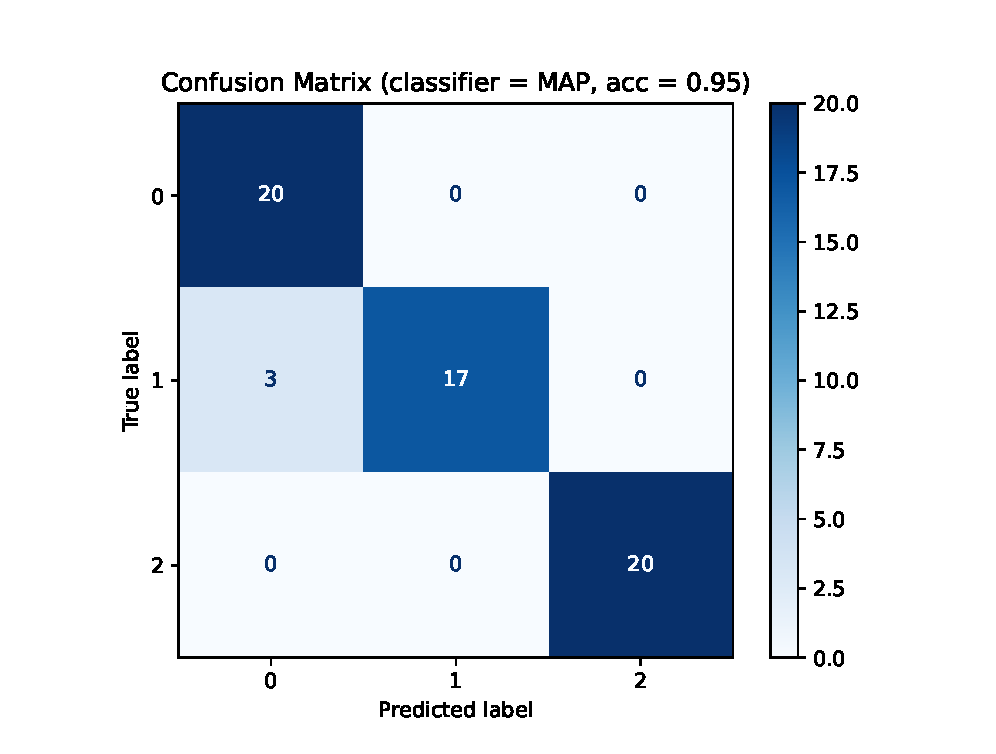
\includegraphics[scale=1.0]{cm_MAP.eps}
        \caption{Confusion matrix of the MAP classifier.}
        \label{fig:cm_map}
    \end{figure}
    \item \textbf{Discussion} \hfill \\
        Below are some key aspects we discussed regarding the dataset and the performance:
\begin{itemize}
    \item \textbf{Data Visualization:}  
    To better understand the distribution of different wine types, we visualize 
    the dataset in both 2D and 3D spaces. The following figures illustrate the 
    feature distribution and potential class separability.
    \begin{figure}[H]
        \centering
        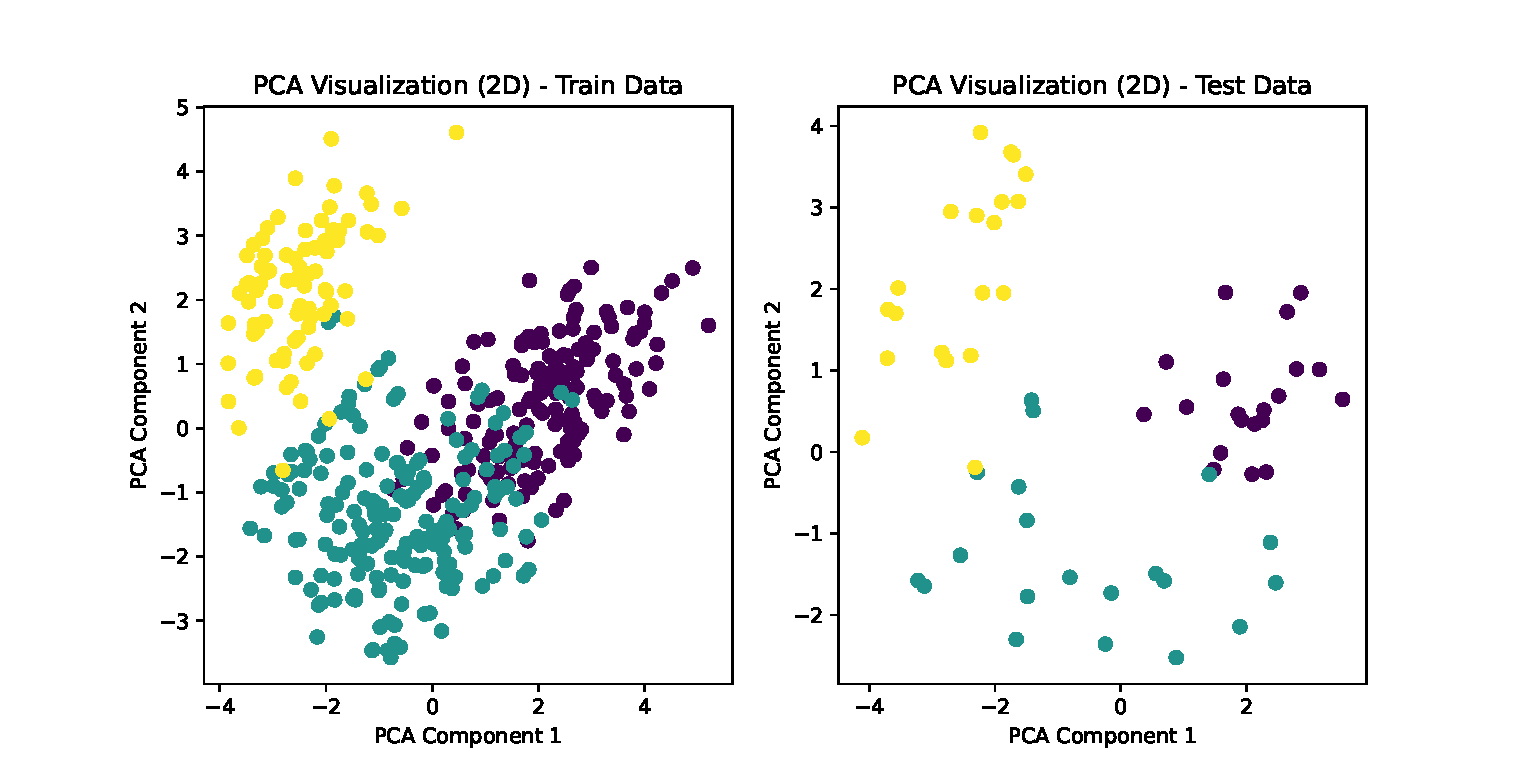
\includegraphics[scale=0.7]{2D_visualize.eps}
        \caption{2D visualization of the dataset.}
        \label{fig:2d_visual}
    \end{figure}
    \begin{figure}[H]
        \centering
        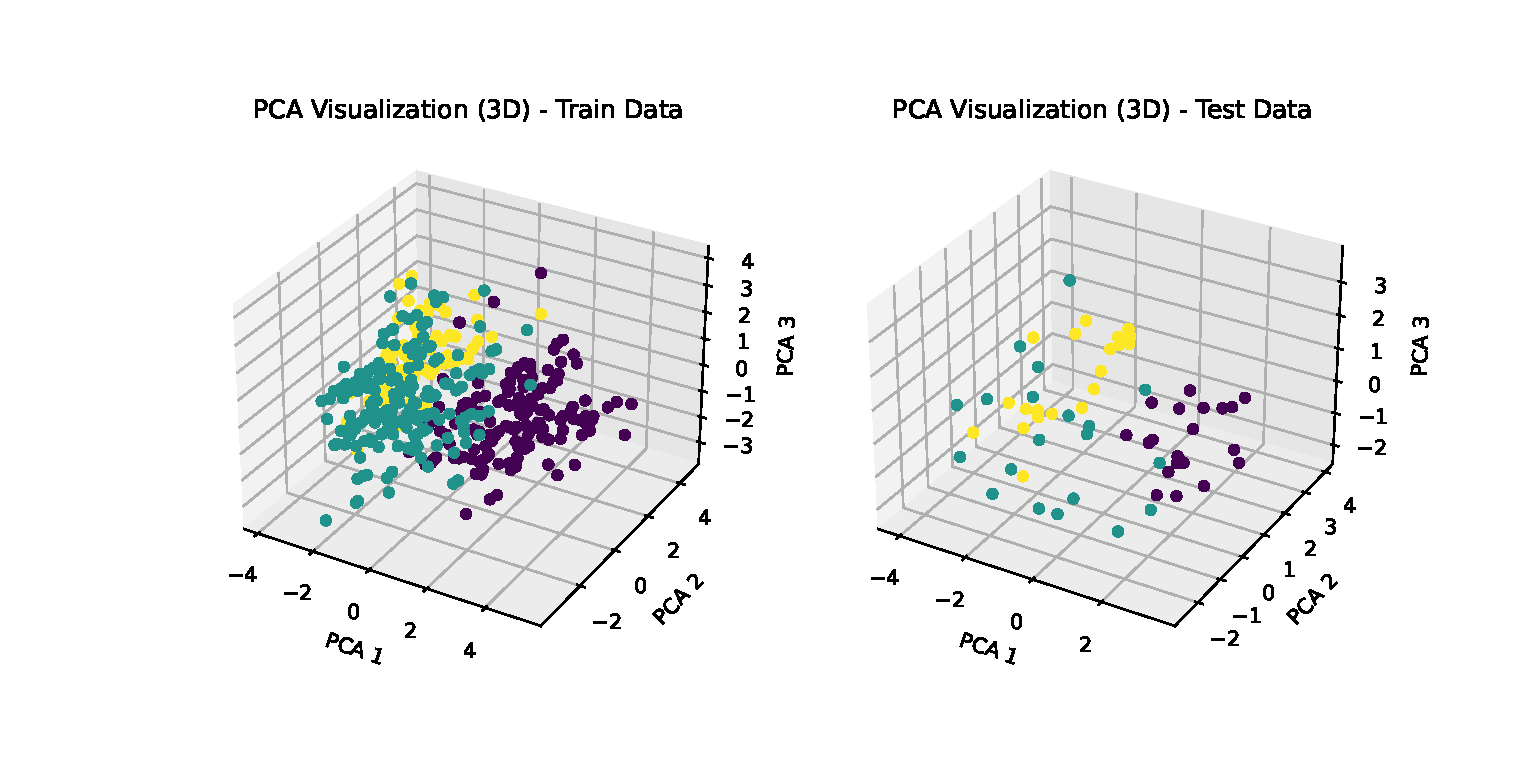
\includegraphics[scale=0.7]{3D_visualize.eps}
        \caption{3D visualization of the dataset.}
        \label{fig:3d_visual}
    \end{figure}
    
    \item \textbf{Effect of Prior Distribution:}  
    To evaluate the influence of prior probabilities on classification performance, 
    we implement a Maximum Likelihood (ML) classifier, which completely disregards 
    prior information. The performance of the ML classifier is shown below:

    \begin{figure}[H]
        \centering
        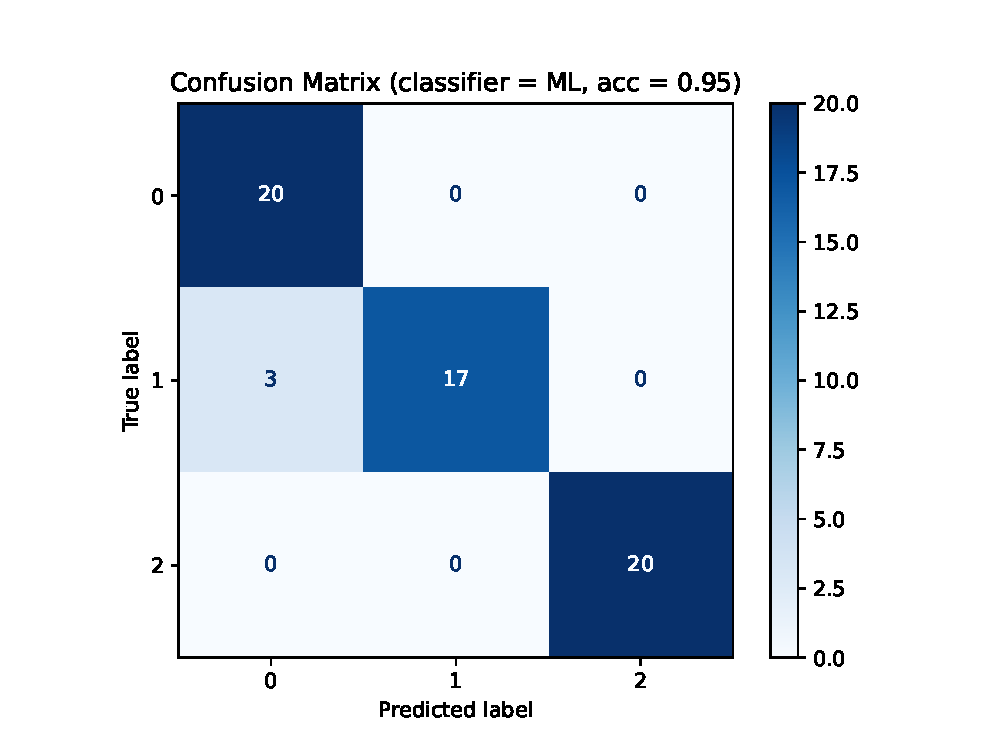
\includegraphics[scale=1.0]{cm_ML.eps}
        \caption{Confusion matrix of the ML classifier.}
        \label{fig:cm_ml}
    \end{figure}

    Interestingly, the results are identical to those obtained with the MAP classifier. 
    This is because, in this problem, the likelihood values are much smaller than the
    prior probabilities. Since the posterior probability is the product of the likelihood 
    and prior, the likelihood becomes the dominant factor, making the effect of the prior 
    negligible.

    \item \textbf{Contribution of Each Feature:} 
    
\end{itemize}

  \end{itemize}
\end{document}